\documentclass[10pt]{article}
\usepackage[a4paper,margin=0.6in,footskip=16pt]{geometry}
\usepackage[T1]{fontenc}
\usepackage{lmodern}
\usepackage[table]{xcolor}
\usepackage{array}
\usepackage{longtable}
\usepackage{enumitem}
\usepackage{amssymb}
\usepackage{amsmath}
\usepackage{graphicx}
\usepackage{adjustbox}
\usepackage{pdflscape}
\usepackage{fancyhdr}
\usepackage{tcolorbox}
\tcbuselibrary{skins}
\usepackage[font=small,labelfont={bf,color=Navy},labelsep=period]{caption}
\usepackage{hyperref}

\newcommand{\doctitle}{TuriTap Handpump Venturi: CFD Analysis}
\newcommand{\currentrev}{1}
\newcommand{\docnumber}{MW-ENG-TT-002}   % TODO: set the real document number
\newcommand{\asof}{Nov 16, 2026}

\newcommand{\rowpad}{1.3}
\definecolor{Navy}{RGB}{11,37,69}
\definecolor{Blue}{RGB}{28,88,152}
\definecolor{LB}{RGB}{232,239,247}
\definecolor{Grey}{RGB}{90,98,110}
\definecolor{StDone}{RGB}{190,230,200}
\definecolor{StProg}{RGB}{255,236,160}
\definecolor{StNS}{RGB}{222,225,229}
\definecolor{MS}{RGB}{255,214,150}
\definecolor{MSDark}{RGB}{214,120,10}
\hypersetup{colorlinks=true, linkcolor=Blue, urlcolor=Blue, citecolor=Blue}

% LOGO: banner.png, looked up in figures/ first, then the project root
\newcommand{\logoimg}[3]{%
  \IfFileExists{figures/#1}{\includegraphics[height=#2,width=#3,keepaspectratio]{figures/#1}}{%
  \IfFileExists{#1}{\includegraphics[height=#2,width=#3,keepaspectratio]{#1}}{}}}
\newcommand{\bannerlogo}[1]{%
  \IfFileExists{figures/banner.png}{\logoimg{banner.png}{#1}{4.5cm}}{%
  \IfFileExists{banner.png}{\logoimg{banner.png}{#1}{4.5cm}}{\textbf{\color{white}MANGROVE WATER}}}}

% HELPERS
\newcommand{\hd}[1]{\textcolor{white}{\textbf{#1}}}
\renewcommand{\arraystretch}{1.3}
\setlength{\arrayrulewidth}{0.4pt}
\arrayrulecolor{Grey!45}
\setlength{\tabcolsep}{4pt}
\setlength{\parindent}{0pt}
\setlength{\parskip}{4pt}
\setlist{nosep,leftmargin=1.4em}
\newcommand{\sectionhead}[1]{{\large\bfseries\color{Navy}#1}\par\vspace{-2pt}{\color{Blue}\rule{\linewidth}{0.8pt}}\par\vspace{3pt}}

% NUMBERED SECTIONS IN THE TEMPLATE STYLE
\newcounter{secn}
\newcounter{subn}[secn]
\renewcommand{\thesubn}{\thesecn.\arabic{subn}}
\newcommand{\numsec}[1]{\par\vspace{6pt}\refstepcounter{secn}\sectionhead{\thesecn\quad #1}}
\newcommand{\subsec}[1]{\par\vspace{5pt}\refstepcounter{subn}{\bfseries\color{Blue}\thesubn\quad #1}\par\vspace{1pt}}
\numberwithin{equation}{secn}
\numberwithin{figure}{secn}
\numberwithin{table}{secn}

% BANNER: \docbanner{title}{subtitle}
\newcommand{\docbanner}[2]{%
\begin{tcolorbox}[colback=Navy,colframe=Navy,arc=0pt,boxrule=0pt,top=9pt,bottom=9pt,left=12pt,right=12pt]
\begin{minipage}[c]{0.62\linewidth}
{\color{white}\fontsize{20}{24}\selectfont\bfseries #1\par}
\vspace{6pt}
{\color{white}#2\par}
\end{minipage}\hfill
\begin{minipage}[c]{0.32\linewidth}
\raggedleft
\bannerlogo{1.7cm}
\end{minipage}
\end{tcolorbox}}

% COMPACT BANNER FOR LANDSCAPE PAGES
\newcommand{\docbannerS}[2]{%
\begin{tcolorbox}[colback=Navy,colframe=Navy,arc=0pt,boxrule=0pt,top=5pt,bottom=5pt,left=12pt,right=12pt]
\begin{minipage}[c]{0.70\linewidth}
{\color{white}\fontsize{17}{20}\selectfont\bfseries #1\par}
\vspace{3pt}
{\color{white}\small #2\par}
\end{minipage}\hfill
\begin{minipage}[c]{0.25\linewidth}
\raggedleft
\bannerlogo{1.2cm}
\end{minipage}
\end{tcolorbox}}

% CALLOUT BOX (same style as the template summary)
\newcommand{\callout}[2]{%
\begin{tcolorbox}[enhanced,colback=LB,colframe=LB,boxrule=0pt,arc=0pt,
  borderline west={3pt}{0pt}{Navy},left=10pt,right=10pt,top=6pt,bottom=6pt]
{\small\bfseries\color{Navy}#1}\par\vspace{2pt}#2
\end{tcolorbox}}

% LANDSCAPE FOOTER
\newcommand{\landfooter}{\vfill
{\small\color{Grey}\docnumber\ \textbar\ Rev.~\currentrev\hfill Mangrove Water\par}}

% TABLE WIDTHS
\setlength{\LTleft}{0pt}
\setlength{\LTright}{0pt}
\newlength{\wFour}
\setlength{\wFour}{\dimexpr\textwidth-8\tabcolsep-5\arrayrulewidth\relax}
\newcommand{\revrow}[4]{#1 & #2 & #3 & #4\\\hline}
\newcommand{\thead}{\rowcolor{Navy}}
\newcolumntype{C}{>{\centering\arraybackslash}p}
\newcommand{\figw}{\linewidth}

\pagestyle{fancy}
\fancyhf{}
\fancyfoot[L]{\small\color{Grey}\docnumber\ \textbar\ Rev.~\currentrev}
\fancyfoot[C]{\small\color{Grey}\thepage}
\fancyfoot[R]{\small\color{Grey}Mangrove Water}
\renewcommand{\headrulewidth}{0pt}

\begin{document}

\docbanner{\doctitle}{Stages 1, 3 and 3b \textbullet{} 2-D axisymmetric RANS \textbullet{} As of \asof{}\\Internal use only. Do not distribute.}

\vspace{4pt}
\callout{SUMMARY}{%
Single-phase, steady RANS simulations (OpenFOAM 13, $k$--$\omega$ SST, wall-resolved, 2-D axisymmetric wedge) of the TuriTap in-line chlorinator Venturi for manual handpumps: the current part, four Stage~3 prototypes and the four printed 1-inch Venturis V1--V4, 54 runs in all from 6 to 50~L/min. All runs converged. \textbf{V3 (18~mm throat) needs the least water level above its inlet at every flow; of the two that keep the 14~mm throat, V4 needs less than V1 at every flow.} The 4$^\circ$ diffuser half-angle removes the wall-flow reversal that covered 47--59\% of prototype B's 5$^\circ$ diffuser at 20--30~L/min. In every design most of the head leaves as kinetic energy in the outlet jet. At 6--8~L/min the chlorine-port suction is set almost entirely by the hanging water column below the port, not by the Venturi, so single-phase CFD cannot predict the dosing cutoff. Elbow and reducer losses are \emph{not} included in any number here.}

\sectionhead{Key result: water level above the Venturi inlet face (cm)}
Negative means the part passes the flow without backing water above its inlet face. Venturi only, straight inflow, no elbow or reducer. Bold marks the lowest of V1--V4 at each flow.

{\centering\rowcolors{2}{white}{LB}
\begin{tabular}{|l|C{1.5cm}|C{1.5cm}|C{1.5cm}|C{1.5cm}|C{1.5cm}|}
\hline
\thead\hd{Design} & \hd{20 L/min} & \hd{25 L/min} & \hd{30 L/min} & \hd{40 L/min} & \hd{50 L/min}\\ \hline
V1 & -5.6 & -2.2 & 1.8 & 11.7 & 23.9\\ \hline
V2 & -8.1 & -6.0 & -3.4 & 3.0 & 10.9\\ \hline
V3 & -9.2 & \textbf{-7.5} & \textbf{-5.4} & \textbf{-0.3} & \textbf{6.2}\\ \hline
V4 & \textbf{-9.2} & -6.2 & -2.7 & 5.8 & 16.4\\ \hline
B\_1in & -3.6 & 0.4 & 5.1 & 16.7 & 31.1\\ \hline

\end{tabular}\par}

\vspace{4pt}
Flow at which the level reaches the inlet face (linear interpolation between simulated flows), V1 / V2 / V3 / V4 / B\_1in: 27.7 / 35.3 / 40.5 / 33.2 / 24.5~L/min.

\vspace{2pt}
\sectionhead{Contents}
\begin{enumerate}[label=\arabic*.]
\item Scope and problem statement \hfill \pageref{sec:scope}
\item Geometry \hfill \pageref{sec:geom}
\item Governing equations and turbulence model \hfill \pageref{sec:eqs}
\item Boundary conditions, numerics and mesh \hfill \pageref{sec:num}
\item Reported quantities and their derivation \hfill \pageref{sec:derive}
\item Verification: convergence, mesh study, 1-D model \hfill \pageref{sec:verify}
\item Results: current part and Stage 3 prototypes \hfill \pageref{sec:res13}
\item Results: printed set V1--V4 (Stage 3b) \hfill \pageref{sec:res3b}
\item Discussion and what to watch \hfill \pageref{sec:disc}
\item Assumptions and limitations \hfill \pageref{sec:limits}
\item Recommendations and next steps \hfill \pageref{sec:next}
\end{enumerate}
Appendix A: every run (landscape) \textbullet{} Appendix B: files, scripts and viewer \textbullet{} Revision history

\newpage
% =====================================================================
\numsec{Scope and problem statement}\label{sec:scope}

The TuriTap Venturi hangs vertically below a manual handpump spout (India Mark~II or Afridev), flow downward, outlet open to atmosphere. Upstream sit a rubber coupler, a reducer and a threaded 90$^\circ$ elbow. A float valve holds the chlorine level with the throat; a needle valve and Teflon tube feed a 1/4-28 port with a 1.67~mm orifice at the throat wall. The current part backs water up until it spills from the pump's overflow holes. The design case is the \emph{average} delivery of about 20--30~L/min (the pump body smooths the piston pulses).

\begin{center}\rowcolors{2}{white}{LB}
\begin{tabular}{|p{0.42\linewidth}|p{0.50\linewidth}|}
\hline
\thead\hd{Known / requirement} & \hd{Value}\\ \hline
Allowable level above Venturi inlet face & about 8.5~cm (Afridev), about 19~cm (India Mark~II), elbow and reducer included \\ \hline
Average handpump delivery & 20--30~L/min \\ \hline
Dosing cutoff (new designs) & at or below 8~L/min \\ \hline
Chlorine port & 1/4-28 thread, 1.67~mm orifice at the throat; must not change \\ \hline
Bench, printed B\_3-4in with cross-vane & dosing starts at 8~L/min; residual 0.4 / 0.5 / 0.81~mg/L at 8 / 15 / 40~L/min \\ \hline
Handpump, printed B\_3-4in & still overflows (24 strokes in 12~s vs 10 in 8~s for the current part; different pumping speeds) \\ \hline
Reducer and elbow alone & no overflow, or only after a long time \\ \hline
\end{tabular}\end{center}

\textbf{Questions answered here.} (i) How much water level does each Venturi need at 20--50~L/min? (ii) Where does that head go: outlet jet or internal loss? (iii) Does the 4$^\circ$ diffuser stay attached where B's 5$^\circ$ diffuser reversed? (iv) How does chlorine-port pressure change with throat size? (v) How far can the single-phase model be trusted?

% =====================================================================
\numsec{Geometry}\label{sec:geom}

Bores are taken from \texttt{geometry/bore\_stations.csv}; $z$ is measured downward from the inlet face. Prototypes A, B and the V-set have tangent fillets (A and B: R10 inlet-to-cone, R14 cone-to-throat, R14 throat-to-diffuser; V-set: R14 and R14 only, no straight inlet, the 20$^\circ$ cone starts at the 31.2~mm inlet face). Half-angles in Table~\ref{tab:geom} are computed from the meshed wall between the diffuser tangent points. V2 and V3 reach the 26~mm exit before the end of the part and finish with a straight tail (V2 from $z=106.4$~mm, V3 from $z=89.3$~mm).

\begin{table}[htbp]\centering\small
\caption{Geometry of every simulated design. $A_t/A_1$: throat-to-inlet area ratio. $A_e/A_t$: exit-to-throat area ratio. $h_\mathrm{col}$: height of the water column from the port axis to the outlet.}\label{tab:geom}
\rowcolors{2}{white}{LB}
\begin{tabular}{|l|r|r|r|r|r|r|r|r|r|}
\hline
\thead\hd{Design} & \hd{$D_1$ (mm)} & \hd{$D_t$ (mm)} & \hd{$D_e$ (mm)} & \hd{$A_t/A_1$} & \hd{$A_e/A_t$} & \hd{$\theta_d$ ($^\circ$)} & \hd{$L$ (mm)} & \hd{$z_\mathrm{port}$ (mm)} & \hd{$h_\mathrm{col}$ (mm)}\\ \hline
Current & 21.5 & 12.3 & 17.2 & 0.324 & 1.96 & 4.8 & 116.5 & 47.50 & 69.0\\ \hline
A\_3-4in & 21.0 & 14.0 & 19.0 & 0.444 & 1.84 & 5.0 & 116.5 & 31.62 & 84.9\\ \hline
A\_1in & 26.6 & 14.0 & 19.0 & 0.277 & 1.84 & 5.0 & 116.5 & 39.31 & 77.2\\ \hline
B\_3-4in & 21.0 & 14.0 & 26.0 & 0.444 & 3.45 & 5.0 & 116.5 & 31.62 & 84.9\\ \hline
B\_1in & 26.6 & 14.0 & 26.0 & 0.277 & 3.45 & 5.0 & 116.5 & 39.31 & 77.2\\ \hline
V1 & 31.2 & 14.0 & 26.0 & 0.201 & 3.45 & 4.0 & 125.0 & 30.63 & 94.4\\ \hline
V2 & 31.2 & 16.0 & 26.0 & 0.263 & 2.64 & 4.0 & 125.0 & 27.88 & 97.1\\ \hline
V3 & 31.2 & 18.0 & 26.0 & 0.333 & 2.09 & 4.0 & 125.0 & 25.13 & 99.9\\ \hline
V4 & 31.2 & 14.0 & 30.0 & 0.201 & 4.59 & 4.0 & 153.0 & 30.63 & 122.4\\ \hline

\end{tabular}
\end{table}

\begin{figure}[htbp]\centering
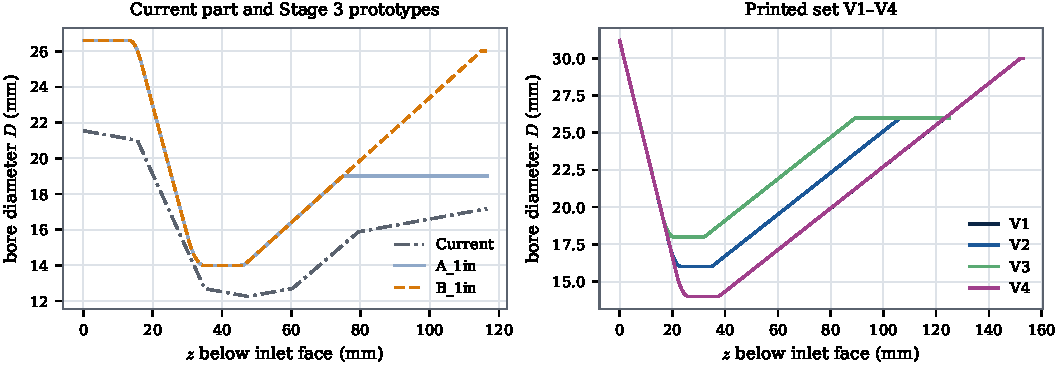
\includegraphics[width=\figw]{figures/bore_profiles.pdf}
\caption{Bore diameter along the axis. The V-set has no straight inlet; V4 is 28~mm longer than V1--V3.}\label{fig:bores}
\end{figure}

% =====================================================================
\numsec{Governing equations and turbulence model}\label{sec:eqs}

\subsec{Flow equations}
Water at 25$^\circ$C is treated as incompressible and Newtonian: $\rho = 997$~kg/m$^3$, $\nu = 8.9\times10^{-7}$~m$^2$/s. The steady Reynolds-averaged equations, with gravity $\mathbf{g} = (9.81, 0, 0)$~m/s$^2$ acting along the flow ($+x$ is downward), are
\begin{align}
\nabla\cdot\mathbf{U} &= 0, \label{eq:cont}\\
\nabla\cdot(\mathbf{U}\mathbf{U}) &= -\frac{1}{\rho}\nabla p + \nabla\cdot\left[(\nu+\nu_t)\left(\nabla\mathbf{U}+\nabla\mathbf{U}^{T}\right)\right] + \mathbf{g}, \label{eq:mom}
\end{align}
where $p$ is the static (gauge) pressure, including its hydrostatic part, and $\nu_t$ is the eddy viscosity. The solver is \texttt{foamRun -solver incompressibleFluid}; gravity enters through the \texttt{buoyancyForce} model, so a column of still water would show $\partial p/\partial x = \rho g$.

\subsec{$k$--$\omega$ SST}
Menter's SST model (1994; OpenFOAM \texttt{kOmegaSST}) solves
\begin{align}
\nabla\cdot(\mathbf{U}k) &= \tilde{P}_k - \beta^* k\omega + \nabla\cdot\left[(\nu + \sigma_k\nu_t)\nabla k\right],\\
\nabla\cdot(\mathbf{U}\omega) &= \frac{\gamma}{\nu_t}\tilde{P}_k - \beta\omega^2 + \nabla\cdot\left[(\nu+\sigma_\omega\nu_t)\nabla\omega\right] + 2(1-F_1)\frac{\sigma_{\omega2}}{\omega}\nabla k\cdot\nabla\omega,\\
\nu_t &= \frac{a_1 k}{\max(a_1\omega,\ S F_2)},\qquad \tilde{P}_k = \min\left(\nu_t S^2,\ 10\beta^* k\omega\right),
\end{align}
with $S$ the strain-rate magnitude, $F_1$, $F_2$ the blending functions, $\beta^* = 0.09$, $a_1 = 0.31$, and inner/outer constants $\beta_1 = 0.075$, $\beta_2 = 0.0828$, $\sigma_{k1}=0.85$, $\sigma_{k2}=1$, $\sigma_{\omega1}=0.5$, $\sigma_{\omega2}=0.856$. The model is integrated to the wall (no wall functions): at 6--12~L/min the near-wall Reynolds numbers are too low for log-law wall functions to hold.

\subsec{Flow regime}
The Reynolds number based on local diameter is $\mathrm{Re} = \bar{V}D/\nu = 4Q/(\pi D\nu)$. Table~\ref{tab:re} shows every run is turbulent at the throat; the lowest values (about 10{,}000 at 6~L/min) are in the transitional-turbulent range where RANS is least reliable.

\begin{table}[htbp]\centering\small
\caption{Reynolds number ($\times 10^3$) at the throat for selected flows, and at the inlet for 25~L/min.}\label{tab:re}
\rowcolors{2}{white}{LB}
\begin{tabular}{|l|r|r|r|r|r|r|}
\hline
\thead\hd{Design} & \hd{6 L/min} & \hd{8 L/min} & \hd{20 L/min} & \hd{30 L/min} & \hd{50 L/min} & \hd{Inlet, 25 L/min}\\ \hline
Current & 11.7 & 15.6 & 38.9 & 58.3 & 97.2 & 27.7\\ \hline
A\_3-4in & 10.2 & 13.6 & 34.1 & 51.1 & 85.2 & 28.4\\ \hline
A\_1in & 10.2 & 13.6 & 34.1 & 51.1 & 85.2 & 22.4\\ \hline
B\_3-4in & 10.2 & 13.6 & 34.1 & 51.1 & 85.2 & 28.4\\ \hline
B\_1in & 10.2 & 13.6 & 34.1 & 51.1 & 85.2 & 22.4\\ \hline
V1 & 10.2 & 13.6 & 34.1 & 51.1 & 85.2 & 19.1\\ \hline
V2 & 8.9 & 11.9 & 29.8 & 44.7 & 74.5 & 19.1\\ \hline
V3 & 7.9 & 10.6 & 26.5 & 39.7 & 66.2 & 19.1\\ \hline
V4 & 10.2 & 13.6 & 34.1 & 51.1 & 85.2 & 19.1\\ \hline

\end{tabular}
\end{table}

% =====================================================================
\numsec{Boundary conditions, numerics and mesh}\label{sec:num}

\subsec{Domain}
A 5$^\circ$ wedge (one cell thick, $\pm2.5^\circ$) of the bore from the inlet face to the outlet face, with \texttt{wedge} patches on the two sides. The elbow, reducer, chlorine port hole and outlet cross-vane are not modelled.

\subsec{Boundary conditions}
\begin{center}\small\rowcolors{2}{white}{LB}
\begin{tabular}{|l|p{0.26\linewidth}|p{0.26\linewidth}|p{0.28\linewidth}|}
\hline
\thead\hd{Field} & \hd{Inlet} & \hd{Outlet (atmosphere)} & \hd{Wall}\\ \hline
$\mathbf{U}$ & uniform, fixed flow rate $Q$ (\texttt{flowRateInletVelocity}) & \texttt{pressureInletOutletVelocity} (backflow-safe) & no slip \\ \hline
$p$ & \texttt{fixedFluxPressure} & \texttt{totalPressure}, $p_0=0$: $p=0$ for outflow, $p=-\tfrac12\rho|\mathbf{U}|^2$ for inflow & \texttt{fixedFluxPressure} \\ \hline
$k$ & $k = \tfrac32(I\bar{V}_1)^2$, $I = 5\%$ & \texttt{inletOutlet} & $k=0$ \\ \hline
$\omega$ & $\omega = \sqrt{k}/(C_\mu^{1/4}\ell)$, $\ell = 0.07D_1$ & \texttt{inletOutlet} & $\omega_w = 10\cdot\dfrac{6\nu}{\beta_1 y_1^2}$ (Menter), per face \\ \hline
$\nu_t$ & calculated & calculated & 0 \\ \hline
\end{tabular}\end{center}
$y_1$ is the distance from the wall to the first cell centre and $C_\mu = 0.09$. The inlet profile is uniform, so area- and flux-weighted inlet averages coincide.

\subsec{Numerics}
Steady SIMPLEC (\texttt{consistent yes}), no non-orthogonal correctors; under-relaxation $\mathbf{U}$ 0.9, $k$ and $\omega$ 0.7. Convection: bounded linear-upwind for $\mathbf{U}$, bounded limited-linear for $k$ and $\omega$; gradients Gauss linear (cell-limited for $k$, $\omega$); Laplacians corrected. Pressure: GAMG, relative tolerance 0.05; others: symmetric Gauss--Seidel, relative tolerance 0.1. Every run is 4000 iterations. Diverging uniform starts at large exits (26--30~mm) were restarted from a plug-flow initial field $U_x = Q/A(z)$ or from a converged neighbouring flow; the converged steady answer does not depend on the initial field, and no setting was changed.

\subsec{Mesh}
A structured, body-fitted quadrilateral mesh is generated directly from the bore table by \texttt{cfd/make\_wedge\_mesh.py}: $n_r$ radial cells graded from the axis to a first cell of height $h_1$ at the wall, axial spacing $h_\mathrm{core}$ refined to $h_\mathrm{corner}$ at fillets and corners with a growth ratio of at most 1.10. The medium mesh is used for every production run. \texttt{checkMesh} passed on every case; maximum non-orthogonality is 20$^\circ$ (limit 65$^\circ$).

\begin{table}[htbp]\centering\small
\caption{Mesh levels (current part, 25~L/min). $h$ values in mm.}\label{tab:mesh}
\rowcolors{2}{white}{LB}
\begin{tabular}{|l|r|r|r|r|r|r|r|r|r|}
\hline
\thead\hd{Level} & \hd{$n_r$} & \hd{$h_\mathrm{core}$} & \hd{$h_\mathrm{corner}$} & \hd{$h_1$ ($\mu$m)} & \hd{Cells} & \hd{$y^+_\mathrm{max}$} & \hd{$y^+_\mathrm{mean}$} & \hd{Non-orth. ($^\circ$)} & \hd{Skewness}\\ \hline
Coarse & 54 & 0.300 & 0.0600 & 4.5 & 25{,}380 & 1.12 & 0.35 & 12.1 & 0.33\\ \hline
Medium & 80 & 0.200 & 0.0400 & 3.0 & 53{,}040 & 0.84 & 0.23 & 12.1 & 0.33\\ \hline
Fine & 120 & 0.133 & 0.0267 & 2.0 & 114{,}480 & 0.63 & 0.16 & 12.1 & 0.33\\ \hline

\end{tabular}
\end{table}

% =====================================================================
\numsec{Reported quantities and their derivation}\label{sec:derive}

Subscript 1 is the inlet face, $t$ the throat, $o$ the outlet face. $\bar{V} = Q/A$ is a section-mean velocity; overbars on pressures are area averages. $\Delta z = L$ is the drop from inlet face to outlet face.

\subsec{Water level above the inlet face (the overflow number)}
Upstream of the Venturi the water stands at rest with a free surface at atmospheric pressure, a height $h$ above the inlet face. The steady energy equation from that free surface to the inlet face, with the upstream fittings' loss $h_{L,\mathrm{up}}$ kept separate, is
\begin{equation}
0 + h = \frac{\bar{p}_1}{\rho g} + \frac{\bar{V}_1^2}{2g} + h_{L,\mathrm{up}}
\quad\Longrightarrow\quad
h = \frac{\bar{p}_{t,1}}{\rho g} + h_{L,\mathrm{up}},\qquad \bar{p}_{t,1} = \frac{1}{A_1}\int_{A_1}\left(p + \tfrac12\rho|\mathbf{U}|^2\right)dA . \label{eq:level}
\end{equation}
The CFD reports $h_\mathrm{CFD} = \bar{p}_{t,1}/(\rho g)$; the elbow and reducer term $h_{L,\mathrm{up}}$ is added by hand. Because gravity is in the momentum equation and the outlet is at $p=0$, $\bar{p}_{t,1}$ already includes the benefit of the column hanging below the inlet.

\subsec{Static pressure at the inlet (air-ingress flag)}
$\bar{p}_1 = \bar{p}_{t,1} - \tfrac12\rho\bar{V}_1^2$. If $\bar{p}_1 < 0$ (gauge) the real part would draw air in at any leak or vent at the inlet joint, and the pipe-full solution is then not physical there. Every such run is flagged (shaded in the tables).

\subsec{Chlorine port pressure}
$p_\mathrm{port}$ is the wall static pressure averaged over the axial span of the 1.67~mm orifice centred on the port axis. It splits naturally into a hydrostatic and a Venturi part. Applying the energy equation along the flow from the port section to the outlet ($p_o = 0$), with section-averaged quantities,
\begin{equation}
\frac{p_\mathrm{port}}{\rho g} + \alpha_t\frac{\bar{V}_t^2}{2g} + h_\mathrm{col} = \alpha_o\frac{\bar{V}_o^2}{2g} + h_{L,\mathrm{port}\to o}
\ \Longrightarrow\
p_\mathrm{port} = \underbrace{-\rho g h_\mathrm{col}}_{\text{hanging column}} \underbrace{-\tfrac12\rho\left(\alpha_t\bar{V}_t^2 - \alpha_o\bar{V}_o^2\right) + \rho g\, h_{L,\mathrm{port}\to o}}_{p_V,\ \text{Venturi part}} . \label{eq:port}
\end{equation}
We report $p_\mathrm{port}$ and $p_V = p_\mathrm{port} + \rho g h_\mathrm{col}$. The hanging-column term exists only while the bore below the port runs full of water.

\subsec{Diffuser pressure recovery}
With $x$ downward, the piezometric pressure is $p^* = p - \rho g x$. Between the diffuser inlet (1d) and exit (2d),
\begin{equation}
C_p = \frac{\bar{p}^*_{2d} - \bar{p}^*_{1d}}{\tfrac12\rho\bar{V}_{1d}^2},\qquad
C_{p,\mathrm{ideal}} = 1 - \left(\frac{A_{1d}}{A_{2d}}\right)^2 = 1 - \left(\frac{D_{1d}}{D_{2d}}\right)^4,\qquad
\eta_d = \frac{C_p}{C_{p,\mathrm{ideal}}}, \label{eq:cp}
\end{equation}
where $C_{p,\mathrm{ideal}}$ follows from Bernoulli and continuity for uniform inviscid flow.

\subsec{Separation}
Wall flow is reversed where the near-wall axial velocity, and so the axial wall shear $\tau_{w,x}$, is negative. The reversed fraction is $\epsilon_\mathrm{rev} = \sum \Delta z_\mathrm{rev} / L_d$ over the wall faces of the diffuser, and the reversed $z$-ranges are listed.

\subsec{Outlet jet energy and the head budget}
The kinetic-energy flux leaving the outlet, written as head, and the energy factor $\alpha$ are
\begin{equation}
h_{KE} = \frac{1}{gQ}\int_{A_o}\tfrac12|\mathbf{U}|^2\,u_x\,dA = \alpha_o\frac{\bar{V}_o^2}{2g},\qquad
\alpha_o = \frac{\int_{A_o}|\mathbf{U}|^2 u_x\,dA}{Q\,\bar{V}_o^2}\ \ (=1\ \text{for uniform flow}). \label{eq:alpha}
\end{equation}
The energy equation from inlet to outlet (datum at the outlet, $p_o = 0$) gives the internal loss:
\begin{equation}
\frac{\bar{p}_{t,1}}{\rho g} + \Delta z = h_{KE} + h_L
\quad\Longrightarrow\quad
h_L = h_\mathrm{CFD} + \Delta z - h_{KE}. \label{eq:budget}
\end{equation}
So the level is $h_\mathrm{CFD} = h_{KE} + h_L - \Delta z$: a longer part (larger $\Delta z$) helps one-for-one, and a lossless part with a uniform exit still needs $\bar{V}_o^2/2g - \Delta z$.

\subsec{Mass balance and convergence measures}
$\epsilon_m = (Q_1 + Q_o)/Q_1$ (outflow negative). A run is judged converged when the final initial residual of $p$ is below $10^{-4}$, the inlet pressure changes by less than $10^{-3}$ (relative) over the last 500 iterations and $|\epsilon_m| < 10^{-4}$. OpenFOAM's \texttt{residualControl} is never met on a wedge because the out-of-plane velocity residual stays near 0.4 (that component is identically zero and its normalised residual is meaningless); it is not used.

\subsec{Mesh uncertainty}
For the three meshes (refinement ratio $r = 1.5$), Roache's grid convergence index uses the observed order and a safety factor $F_s = 1.25$:
\begin{equation}
p_\mathrm{obs} = \frac{\ln\left|(f_2-f_3)/(f_1-f_2)\right|}{\ln r},\qquad
\mathrm{GCI}_\mathrm{fine} = \frac{F_s\,|(f_1-f_2)/f_1|}{r^{p_\mathrm{obs}}-1}, \label{eq:gci}
\end{equation}
with $f_1$ fine, $f_2$ medium, $f_3$ coarse.

% =====================================================================
\numsec{Verification: convergence, mesh study, 1-D model}\label{sec:verify}

\subsec{Convergence}
All 54 runs reached 4000 iterations and meet every criterion of Section~\ref{sec:derive} (Table~\ref{tab:conv}). Fig.~\ref{fig:conv} shows a typical history: the inlet pressure settles to within 1\% of its final value in about 800--900 iterations.

\begin{table}[htbp]\centering\small
\caption{Worst-case convergence measures per design (over all its runs).}\label{tab:conv}
\rowcolors{2}{white}{LB}
\begin{tabular}{|l|r|r|r|r|r|}
\hline
\thead\hd{Design} & \hd{Runs} & \hd{max $p$ residual} & \hd{max inlet $\Delta p$, last 500} & \hd{max $|\epsilon_m|$} & \hd{max $y^+$}\\ \hline
Current & 8 & $1.2\times10^{-6}$ & $2.0\times10^{-6}$ & $2.6\times10^{-9}$ & 1.12\\ \hline
A\_3-4in & 6 & $2.1\times10^{-7}$ & $5.0\times10^{-8}$ & $2.2\times10^{-10}$ & 0.85\\ \hline
A\_1in & 6 & $4.2\times10^{-7}$ & $1.3\times10^{-6}$ & $3.4\times10^{-9}$ & 0.76\\ \hline
B\_3-4in & 6 & $7.0\times10^{-8}$ & $1.1\times10^{-7}$ & $8.7\times10^{-11}$ & 0.85\\ \hline
B\_1in & 8 & $3.3\times10^{-7}$ & $1.0\times10^{-6}$ & $3.3\times10^{-9}$ & 1.09\\ \hline
V1 & 5 & $4.3\times10^{-7}$ & $2.1\times10^{-5}$ & $1.4\times10^{-8}$ & 1.07\\ \hline
V2 & 5 & $2.0\times10^{-7}$ & $5.2\times10^{-6}$ & $3.7\times10^{-9}$ & 0.94\\ \hline
V3 & 5 & $3.3\times10^{-7}$ & $7.7\times10^{-6}$ & $1.6\times10^{-9}$ & 0.84\\ \hline
V4 & 5 & $4.4\times10^{-7}$ & $3.1\times10^{-5}$ & $2.0\times10^{-8}$ & 1.07\\ \hline

\end{tabular}
\end{table}

\begin{figure}[htbp]\centering
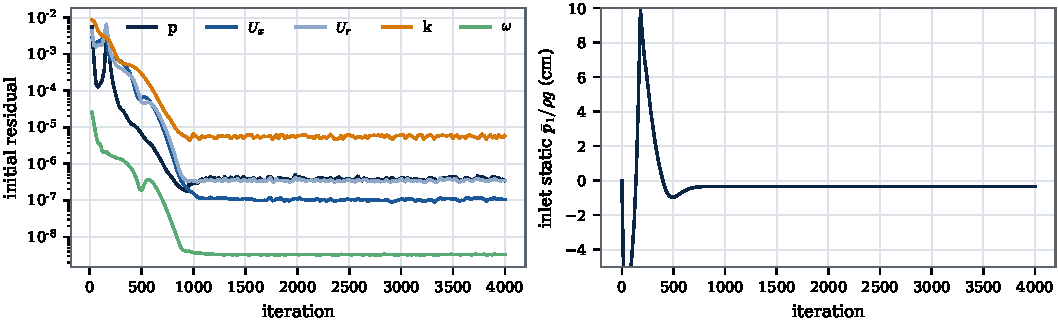
\includegraphics[width=\figw]{figures/convergence_V1_30.pdf}
\caption{V1 at 30~L/min. Left: initial residuals ($U_r$ is the radial component). Right: area-averaged inlet static pressure, as head.}\label{fig:conv}
\end{figure}

\subsec{Mesh study}
Current part at 25~L/min on three meshes (Table~\ref{tab:mesh}). Every tracked quantity changes by at most 1.2\% from coarse to medium and under 1\% from medium to fine (Table~\ref{tab:gci}); the level's mesh uncertainty is about 2\%, or 0.35~cm. The medium mesh is adequate. The observed order is below the nominal second order, which is common when the solution has corners (fillet tangency points) and when changes are this small.

\begin{table}[htbp]\centering\small
\caption{Mesh study, current part, 25~L/min. $^\dagger$Non-monotonic; the GCI column then gives $1.25\times$ the largest change.}\label{tab:gci}
\rowcolors{2}{white}{LB}
\begin{tabular}{|l|r|r|r|r|r|r|r|}
\hline
\thead\hd{Quantity} & \hd{Coarse} & \hd{Medium} & \hd{Fine} & \hd{C$\to$M (\%)} & \hd{M$\to$F (\%)} & \hd{$p_\mathrm{obs}$} & \hd{GCI (\%)}\\ \hline
Level above inlet (cm) & 15.42 & 15.53 & 15.61 & +0.69 & +0.53 & 0.64 & 2.25\\ \hline
Inlet static pressure (Pa) & 856 & 867 & 875 & +1.20 & +0.93 & 0.64 & 3.92\\ \hline
Port wall pressure (kPa) & -4.814 & -4.806 & -4.800 & +0.17 & +0.13 & 0.70 & 0.50\\ \hline
Minimum wall pressure (kPa) & -5.979 & -5.981 & -5.971 & -0.03 & +0.16 & osc. & 0.20$^\dagger$\\ \hline
Diffuser recovery (--) & 0.794 & 0.792 & 0.791 & -0.20 & -0.17 & 0.46 & 1.01\\ \hline
Outlet jet head (cm) & 20.55 & 20.59 & 20.62 & +0.21 & +0.15 & 0.74 & 0.55\\ \hline
Outlet $\alpha$ (--) & 1.245 & 1.247 & 1.249 & +0.21 & +0.15 & 0.74 & 0.55\\ \hline

\end{tabular}
\end{table}

\begin{figure}[htbp]\centering
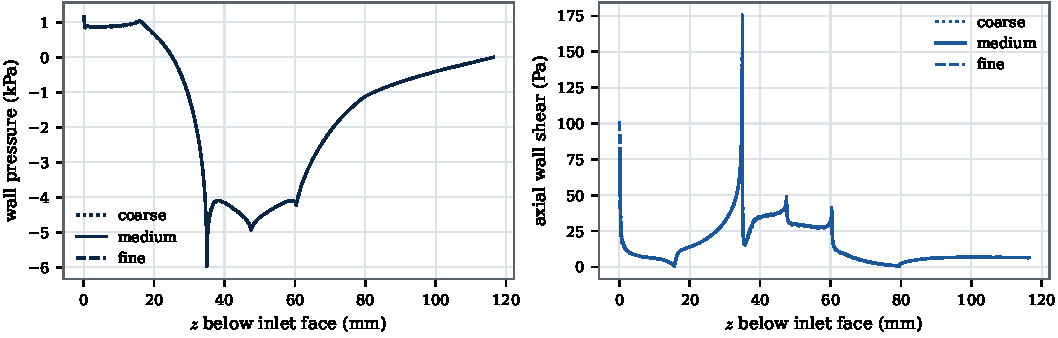
\includegraphics[width=\figw]{figures/mesh_study.pdf}
\caption{Wall pressure and axial wall shear on the three meshes (current part, 25~L/min).}\label{fig:mesh}
\end{figure}

\subsec{Comparison with the 1-D model}
The 1-D model (\texttt{analysis/turitap\_venturi\_analysis.m}: Bernoulli plus handbook loss coefficients, about $\pm25\%$ on losses) is compared with the CFD for the current part in Table~\ref{tab:oned}. Port pressure agrees within 3\%. The CFD level is 17--22\% lower than the 1-D level at 20--30~L/min, beyond the 15\% reporting threshold, but within the 1-D model's stated loss uncertainty. Nothing was tuned to match.

\begin{table}[htbp]\centering\small
\caption{Current part: CFD vs 1-D model (Venturi only).}\label{tab:oned}
\rowcolors{2}{white}{LB}
\begin{tabular}{|r|r|r|r|r|r|r|c|}
\hline
\thead\hd{$Q$ (L/min)} & \hd{1-D level (cm)} & \hd{CFD level (cm)} & \hd{$\Delta$ (\%)} & \hd{1-D port (kPa)} & \hd{CFD port (kPa)} & \hd{$\Delta$ (\%)} & \hd{$>15\%$?}\\ \hline
6 & below inlet & -9.7 & -- & -0.90 & -0.90 & +0 & no\\ \hline
8 & below inlet & -8.4 & -- & -1.07 & -1.08 & -1 & no\\ \hline
20 & 8 & 6.2 & -22 & -3.20 & -3.30 & -3 & \textbf{yes}\\ \hline
25 & 19 & 15.5 & -18 & -4.70 & -4.81 & -2 & \textbf{yes}\\ \hline
30 & 32 & 26.7 & -17 & -6.50 & -6.67 & -3 & \textbf{yes}\\ \hline

\end{tabular}
\end{table}

% =====================================================================
\numsec{Results: current part and Stage 3 prototypes}\label{sec:res13}

Columns in Tables~\ref{tab:rescur}--\ref{tab:resvset}: level $h_\mathrm{CFD}$ (cm), inlet static pressure $\bar{p}_1$ (Pa, shaded when negative), port pressure (kPa), diffuser recovery $\eta_d$, reversed diffuser wall $\epsilon_\mathrm{rev}$ (\%), outlet jet head $h_{KE}$ (cm), $\alpha_o$, internal loss $h_L$ (cm).

\begin{table}[htbp]\centering\small
\caption{Current part, Stage 1 (medium mesh).}\label{tab:rescur}
\rowcolors{2}{white}{LB}
\begin{tabular}{|l|r|r|r|r|r|r|r|r|r|}
\hline
\thead\hd{Design} & \hd{$Q$} & \hd{$h$} & \hd{$\bar{p}_1$} & \hd{$p_\mathrm{port}$} & \hd{$\eta_d$} & \hd{$\epsilon_\mathrm{rev}$} & \hd{$h_{KE}$} & \hd{$\alpha_o$} & \hd{$h_L$}\\ \hline
Current & 6 & -9.70 & \cellcolor{StProg}-986 & -0.898 & 0.694 & 85 & 1.35 & 1.42 & 0.60\\ \hline
Current & 8 & -8.39 & \cellcolor{StProg}-887 & -1.080 & 0.718 & 72 & 2.31 & 1.37 & 0.95\\ \hline
Current & 12 & -4.78 & \cellcolor{StProg}-618 & -1.599 & 0.748 & 25 & 5.01 & 1.32 & 1.86\\ \hline
Current & 20 & 6.21 & 190 & -3.295 & 0.779 & 0 & 13.38 & 1.27 & 4.48\\ \hline
Current & 25 & 15.53 & 867 & -4.806 & 0.792 & 0 & 20.59 & 1.25 & 6.59\\ \hline
Current & 30 & 26.68 & 1671 & -6.666 & 0.802 & 0 & 29.30 & 1.23 & 9.03\\ \hline

\end{tabular}
\end{table}

\begin{table}[htbp]\centering\small
\caption{Stage 3 prototypes at 20--30~L/min (6--12~L/min in Appendix~A).}\label{tab:resproto}
\rowcolors{2}{white}{LB}
\begin{tabular}{|l|r|r|r|r|r|r|r|r|r|}
\hline
\thead\hd{Design} & \hd{$Q$} & \hd{$h$} & \hd{$\bar{p}_1$} & \hd{$p_\mathrm{port}$} & \hd{$\eta_d$} & \hd{$\epsilon_\mathrm{rev}$} & \hd{$h_{KE}$} & \hd{$\alpha_o$} & \hd{$h_L$}\\ \hline
A\_3-4in & 20 & -0.90 & \cellcolor{StProg}-549 & -2.299 & 0.822 & 4 & 8.21 & 1.17 & 2.54\\ \hline
A\_3-4in & 25 & 4.72 & \cellcolor{StProg}-260 & -3.138 & 0.833 & 0 & 12.67 & 1.15 & 3.70\\ \hline
A\_3-4in & 30 & 11.47 & 83 & -4.172 & 0.842 & 0 & 18.08 & 1.14 & 5.03\\ \hline
A\_1in & 20 & -1.01 & \cellcolor{StProg}-278 & -2.234 & 0.823 & 5 & 8.29 & 1.18 & 2.35\\ \hline
A\_1in & 25 & 4.57 & 167 & -3.067 & 0.833 & 0 & 12.79 & 1.16 & 3.43\\ \hline
A\_1in & 30 & 11.27 & 698 & -4.098 & 0.841 & 0 & 18.25 & 1.15 & 4.67\\ \hline
B\_3-4in & 20 & -3.87 & \cellcolor{StProg}-840 & -2.590 & 0.809 & 58 & 4.81 & 2.39 & 2.97\\ \hline
B\_3-4in & 25 & -0.01 & \cellcolor{StProg}-723 & -3.601 & 0.817 & 51 & 7.30 & 2.33 & 4.34\\ \hline
B\_3-4in & 30 & 4.54 & \cellcolor{StProg}-595 & -4.849 & 0.822 & 46 & 10.28 & 2.27 & 5.92\\ \hline
B\_1in & 20 & -3.62 & \cellcolor{StProg}-534 & -2.489 & 0.808 & 59 & 5.32 & 2.65 & 2.70\\ \hline
B\_1in & 25 & 0.38 & \cellcolor{StProg}-243 & -3.476 & 0.815 & 52 & 8.08 & 2.58 & 3.95\\ \hline
B\_1in & 30 & 5.12 & 98 & -4.699 & 0.820 & 47 & 11.38 & 2.52 & 5.40\\ \hline

\end{tabular}
\end{table}

Findings that set up Stage 3b: (i) in every design most of the head leaves as the outlet jet (current part 20.6~cm of 27~cm total at 25~L/min); (ii) the internal loss of A and B is only about 4~cm at 25~L/min; (iii) inlet size (3/4" vs 1") barely changes the Venturi alone; (iv) B's 5$^\circ$ diffuser reverses over about half its wall at 20--30~L/min with $\alpha_o \approx 2.5$.

% =====================================================================
\numsec{Results: printed set V1--V4 (Stage 3b)}\label{sec:res3b}

Same setup as Stage 1, unchanged, at 20, 25, 30, 40 and 50~L/min, plus B\_1in at 40 and 50~L/min for comparison.

\begin{table}[htbp]\centering\small
\caption{V1--V4 and B\_1in, all flows.}\label{tab:resvset}
\rowcolors{2}{white}{LB}
\begin{tabular}{|l|r|r|r|r|r|r|r|r|r|}
\hline
\thead\hd{Design} & \hd{$Q$} & \hd{$h$} & \hd{$\bar{p}_1$} & \hd{$p_\mathrm{port}$} & \hd{$\eta_d$} & \hd{$\epsilon_\mathrm{rev}$} & \hd{$h_{KE}$} & \hd{$\alpha_o$} & \hd{$h_L$}\\ \hline
V1 & 20 & -5.62 & \cellcolor{StProg}-644 & -2.780 & 0.865 & 0 & 4.15 & 2.07 & 2.73\\ \hline
V1 & 25 & -2.20 & \cellcolor{StProg}-364 & -3.822 & 0.870 & 0 & 6.29 & 2.00 & 4.01\\ \hline
V1 & 30 & 1.83 & \cellcolor{StProg}-34 & -5.116 & 0.874 & 0 & 8.84 & 1.96 & 5.49\\ \hline
V1 & 40 & 11.70 & 765 & -8.444 & 0.882 & 0 & 15.14 & 1.88 & 9.06\\ \hline
V1 & 50 & 23.87 & 1743 & -12.759 & 0.887 & 0 & 23.00 & 1.83 & 13.37\\ \hline
V2 & 20 & -8.14 & \cellcolor{StProg}-891 & -2.025 & 0.881 & 0 & 2.77 & 1.38 & 1.58\\ \hline
V2 & 25 & -5.96 & \cellcolor{StProg}-731 & -2.625 & 0.887 & 0 & 4.22 & 1.34 & 2.32\\ \hline
V2 & 30 & -3.37 & \cellcolor{StProg}-543 & -3.364 & 0.892 & 0 & 5.95 & 1.32 & 3.18\\ \hline
V2 & 40 & 3.01 & \cellcolor{StProg}-85 & -5.273 & 0.900 & 0 & 10.27 & 1.28 & 5.23\\ \hline
V2 & 50 & 10.94 & 478 & -7.745 & 0.907 & 0 & 15.72 & 1.25 & 7.72\\ \hline
V3 & 20 & -9.18 & \cellcolor{StProg}-993 & -1.603 & 0.900 & 0 & 2.30 & 1.15 & 1.02\\ \hline
V3 & 25 & -7.47 & \cellcolor{StProg}-878 & -1.949 & 0.907 & 0 & 3.54 & 1.13 & 1.49\\ \hline
V3 & 30 & -5.41 & \cellcolor{StProg}-743 & -2.372 & 0.912 & 0 & 5.04 & 1.12 & 2.04\\ \hline
V3 & 40 & -0.29 & \cellcolor{StProg}-408 & -3.466 & 0.919 & 0 & 8.83 & 1.10 & 3.37\\ \hline
V3 & 50 & 6.15 & 10 & -4.882 & 0.925 & 0 & 13.66 & 1.09 & 4.99\\ \hline
V4 & 20 & -9.22 & \cellcolor{StProg}-996 & -3.132 & 0.868 & 3 & 2.99 & 2.64 & 3.09\\ \hline
V4 & 25 & -6.23 & \cellcolor{StProg}-757 & -4.216 & 0.872 & 0 & 4.53 & 2.56 & 4.54\\ \hline
V4 & 30 & -2.71 & \cellcolor{StProg}-478 & -5.560 & 0.876 & 0 & 6.37 & 2.50 & 6.22\\ \hline
V4 & 40 & 5.85 & 193 & -9.016 & 0.883 & 0 & 10.90 & 2.40 & 10.25\\ \hline
V4 & 50 & 16.37 & 1009 & -13.492 & 0.888 & 0 & 16.55 & 2.34 & 15.12\\ \hline
B\_1in & 20 & -3.62 & \cellcolor{StProg}-534 & -2.489 & 0.808 & 59 & 5.32 & 2.65 & 2.70\\ \hline
B\_1in & 25 & 0.38 & \cellcolor{StProg}-243 & -3.476 & 0.815 & 52 & 8.08 & 2.58 & 3.95\\ \hline
B\_1in & 30 & 5.12 & 98 & -4.699 & 0.820 & 47 & 11.38 & 2.52 & 5.40\\ \hline
B\_1in & 40 & 16.73 & 919 & -7.847 & 0.829 & 38 & 19.53 & 2.43 & 8.85\\ \hline
B\_1in & 50 & 31.08 & 1919 & -11.933 & 0.836 & 30 & 29.72 & 2.37 & 13.00\\ \hline

\end{tabular}
\end{table}

\begin{figure}[htbp]\centering
\begin{minipage}{0.49\linewidth}\centering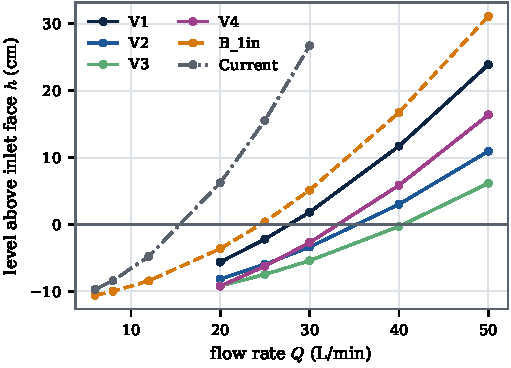
\includegraphics[width=\linewidth]{figures/level_vs_q.pdf}\end{minipage}\hfill
\begin{minipage}{0.49\linewidth}\centering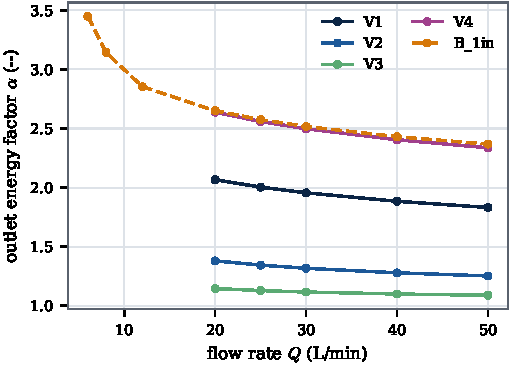
\includegraphics[width=\linewidth]{figures/alpha_vs_q.pdf}\end{minipage}
\caption{Left: level above the inlet face vs flow. Right: outlet energy factor $\alpha_o$.}\label{fig:level}
\end{figure}

\subsec{Head budget}
Eq.~\eqref{eq:budget} splits the available head $h + \Delta z$ into outlet jet and internal loss (Table~\ref{tab:budget}, Fig.~\ref{fig:budget}). V3's advantage comes from both terms: the wide throat cuts internal loss to about 2~cm at 30~L/min, and the nearly uniform exit ($\alpha_o \approx 1.1$) keeps the jet close to its minimum $\bar V_o^2/2g$. V1 has the same exit area as V3, but its jet carries nearly twice the energy because its exit profile is peaked ($\alpha_o\approx2$). V4's 30~mm exit lowers $\bar{V}_o$, but $\alpha_o \approx 2.5$ cancels much of that gain; its lower level comes mostly from its extra 2.8~cm of drop.

\begin{table}[htbp]\centering\small
\caption{Head budget (cm). Available $= h + \Delta z$; shares in \% of available.}\label{tab:budget}
\rowcolors{2}{white}{LB}
\begin{tabular}{|l|r|r|r|r|r|r|r|r|r|}
\hline
\thead\hd{Design} & \hd{$Q$} & \hd{$\Delta z$} & \hd{$h$} & \hd{Available} & \hd{$h_{KE}$} & \hd{Jet \%} & \hd{$h_L$} & \hd{Loss \%} & \hd{$\alpha_o$}\\ \hline
V1 & 20 & 12.5 & -5.62 & 6.88 & 4.15 & 60 & 2.73 & 40 & 2.07\\ \hline
V1 & 25 & 12.5 & -2.20 & 10.30 & 6.29 & 61 & 4.01 & 39 & 2.00\\ \hline
V1 & 30 & 12.5 & +1.83 & 14.33 & 8.84 & 62 & 5.49 & 38 & 1.96\\ \hline
V1 & 40 & 12.5 & +11.70 & 24.20 & 15.14 & 63 & 9.06 & 37 & 1.88\\ \hline
V1 & 50 & 12.5 & +23.87 & 36.37 & 23.00 & 63 & 13.37 & 37 & 1.83\\ \hline
V2 & 20 & 12.5 & -8.14 & 4.36 & 2.77 & 64 & 1.58 & 36 & 1.38\\ \hline
V2 & 25 & 12.5 & -5.96 & 6.54 & 4.22 & 64 & 2.32 & 36 & 1.34\\ \hline
V2 & 30 & 12.5 & -3.37 & 9.13 & 5.95 & 65 & 3.18 & 35 & 1.32\\ \hline
V2 & 40 & 12.5 & +3.01 & 15.51 & 10.27 & 66 & 5.23 & 34 & 1.28\\ \hline
V2 & 50 & 12.5 & +10.94 & 23.44 & 15.72 & 67 & 7.72 & 33 & 1.25\\ \hline
V3 & 20 & 12.5 & -9.18 & 3.32 & 2.30 & 69 & 1.02 & 31 & 1.15\\ \hline
V3 & 25 & 12.5 & -7.47 & 5.03 & 3.54 & 70 & 1.49 & 30 & 1.13\\ \hline
V3 & 30 & 12.5 & -5.41 & 7.09 & 5.04 & 71 & 2.04 & 29 & 1.12\\ \hline
V3 & 40 & 12.5 & -0.29 & 12.21 & 8.83 & 72 & 3.37 & 28 & 1.10\\ \hline
V3 & 50 & 12.5 & +6.15 & 18.65 & 13.66 & 73 & 4.99 & 27 & 1.09\\ \hline
V4 & 20 & 15.3 & -9.22 & 6.08 & 2.99 & 49 & 3.09 & 51 & 2.64\\ \hline
V4 & 25 & 15.3 & -6.23 & 9.07 & 4.53 & 50 & 4.54 & 50 & 2.56\\ \hline
V4 & 30 & 15.3 & -2.71 & 12.59 & 6.37 & 51 & 6.22 & 49 & 2.50\\ \hline
V4 & 40 & 15.3 & +5.85 & 21.15 & 10.90 & 52 & 10.25 & 48 & 2.40\\ \hline
V4 & 50 & 15.3 & +16.37 & 31.67 & 16.55 & 52 & 15.12 & 48 & 2.34\\ \hline
B\_1in & 20 & 11.7 & -3.62 & 8.03 & 5.32 & 66 & 2.70 & 34 & 2.65\\ \hline
B\_1in & 25 & 11.7 & +0.38 & 12.03 & 8.08 & 67 & 3.95 & 33 & 2.58\\ \hline
B\_1in & 30 & 11.7 & +5.12 & 16.77 & 11.38 & 68 & 5.40 & 32 & 2.52\\ \hline
B\_1in & 40 & 11.7 & +16.73 & 28.38 & 19.53 & 69 & 8.85 & 31 & 2.43\\ \hline
B\_1in & 50 & 11.7 & +31.08 & 42.73 & 29.72 & 70 & 13.00 & 30 & 2.37\\ \hline

\end{tabular}
\end{table}

\begin{figure}[htbp]\centering
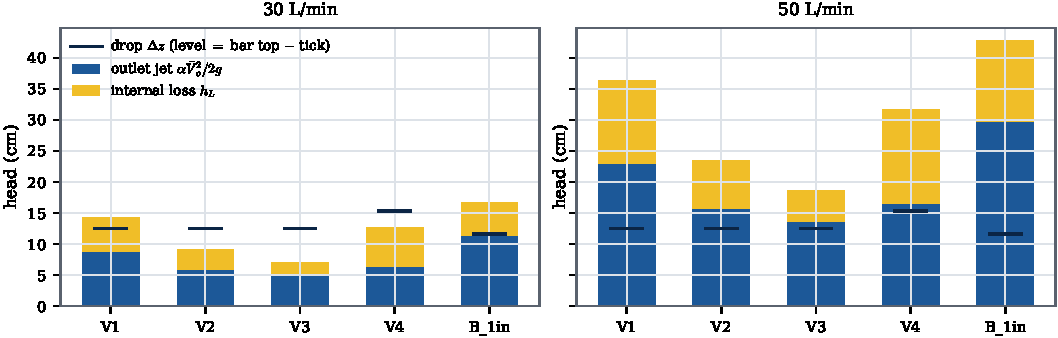
\includegraphics[width=\figw]{figures/head_budget.pdf}
\caption{Head budget at 30 and 50~L/min. Bar height is the available head $h+\Delta z$; the dark tick is $\Delta z$, so the level is the bar top minus the tick.}\label{fig:budget}
\end{figure}

\subsec{Diffuser behaviour}
No reversed wall flow occurs in V1, V2 or V3 at any flow. V4 reverses only in the last 3~mm before the outlet at 20~L/min and in a 0.1~mm sliver at 25~L/min. B\_1in reverses over 59\% of its diffuser wall at 20~L/min, falling to 30\% at 50~L/min (Table~\ref{tab:diff}, Fig.~\ref{fig:shear}). V1's diffuser is attached but marginal: its wall shear falls to about 0.3~Pa at the exit at 30~L/min.

\begin{table}[htbp]\centering\small
\caption{Diffuser recovery and separation.}\label{tab:diff}
\rowcolors{2}{white}{LB}
\begin{tabular}{|l|r|r|r|r|r|r|p{0.22\linewidth}|}
\hline
\thead\hd{Design} & \hd{$Q$} & \hd{$C_p$} & \hd{$C_{p,\mathrm{ideal}}$} & \hd{$\eta_d$} & \hd{min $\tau_{w,x}$ (Pa)} & \hd{$\epsilon_\mathrm{rev}$ (\%)} & \hd{Reversed $z$ (mm)}\\ \hline
V1 & 20 & 0.791 & 0.915 & 0.865 & 0.01 & 0 & none\\ \hline
V1 & 25 & 0.796 & 0.915 & 0.870 & 0.05 & 0 & none\\ \hline
V1 & 30 & 0.800 & 0.915 & 0.874 & 0.12 & 0 & none\\ \hline
V1 & 40 & 0.807 & 0.915 & 0.882 & 0.30 & 0 & none\\ \hline
V1 & 50 & 0.812 & 0.915 & 0.887 & 0.56 & 0 & none\\ \hline
V2 & 20 & 0.754 & 0.856 & 0.881 & 0.09 & 0 & none\\ \hline
V2 & 25 & 0.759 & 0.856 & 0.887 & 0.18 & 0 & none\\ \hline
V2 & 30 & 0.763 & 0.856 & 0.892 & 0.29 & 0 & none\\ \hline
V2 & 40 & 0.770 & 0.856 & 0.900 & 0.59 & 0 & none\\ \hline
V2 & 50 & 0.776 & 0.856 & 0.907 & 0.98 & 0 & none\\ \hline
V3 & 20 & 0.692 & 0.769 & 0.900 & 0.22 & 0 & none\\ \hline
V3 & 25 & 0.697 & 0.769 & 0.907 & 0.37 & 0 & none\\ \hline
V3 & 30 & 0.701 & 0.769 & 0.912 & 0.56 & 0 & none\\ \hline
V3 & 40 & 0.707 & 0.769 & 0.919 & 1.04 & 0 & none\\ \hline
V3 & 50 & 0.711 & 0.769 & 0.925 & 1.65 & 0 & none\\ \hline
V4 & 20 & 0.827 & 0.952 & 0.868 & -0.02 & 3 & 148.8--152.2\\ \hline
V4 & 25 & 0.831 & 0.952 & 0.872 & -0.00 & 0 & 152.0--152.1\\ \hline
V4 & 30 & 0.834 & 0.952 & 0.876 & 0.03 & 0 & none\\ \hline
V4 & 40 & 0.840 & 0.952 & 0.883 & 0.12 & 0 & none\\ \hline
V4 & 50 & 0.845 & 0.952 & 0.888 & 0.24 & 0 & none\\ \hline
B\_1in & 20 & 0.739 & 0.915 & 0.808 & -0.30 & 59 & 74.7--116.5\\ \hline
B\_1in & 25 & 0.746 & 0.915 & 0.815 & -0.38 & 52 & 79.1--116.3\\ \hline
B\_1in & 30 & 0.751 & 0.915 & 0.820 & -0.45 & 47 & 82.9--116.3\\ \hline
B\_1in & 40 & 0.759 & 0.915 & 0.829 & -0.58 & 38 & 89.1--116.3\\ \hline
B\_1in & 50 & 0.765 & 0.915 & 0.836 & -0.70 & 30 & 94.3--116.0, 116.1--116.3\\ \hline

\end{tabular}
\end{table}

\begin{figure}[htbp]\centering
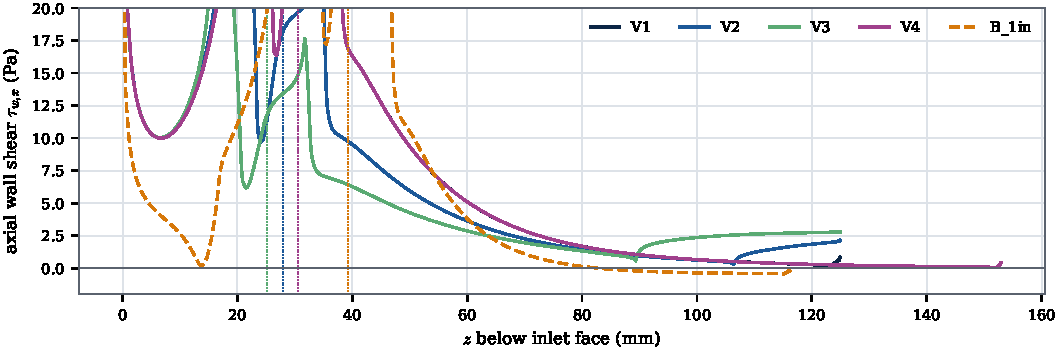
\includegraphics[width=\figw]{figures/wall_shear_30.pdf}
\caption{Axial wall shear at 30~L/min (dotted lines: port positions). Below zero the wall flow runs upstream. Only B\_1in crosses zero, over $z \approx 83$--$116$~mm.}\label{fig:shear}
\end{figure}

\begin{figure}[htbp]\centering
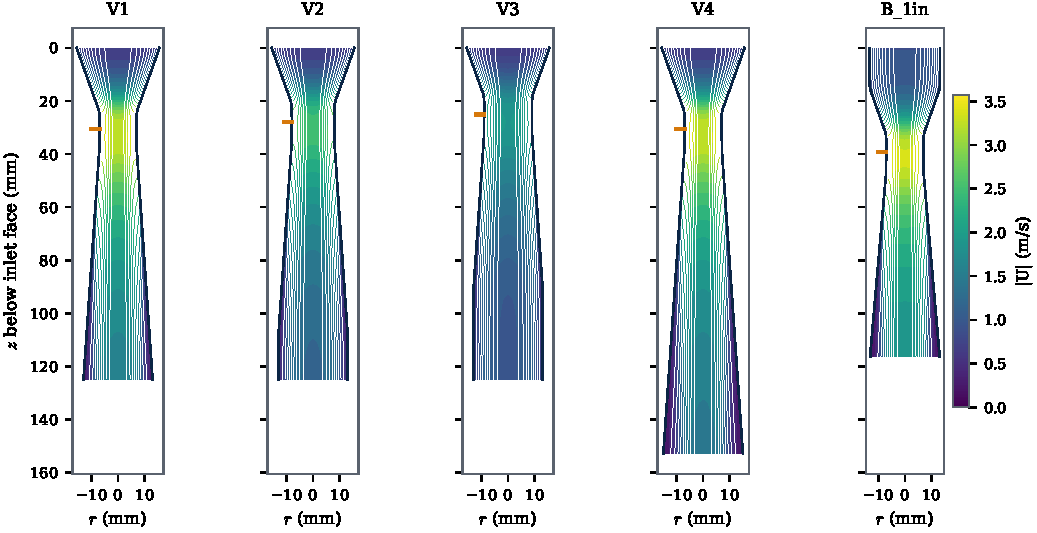
\includegraphics[width=\figw]{figures/speed_cuts_30.pdf}
\caption{Velocity magnitude on the meridional plane at 30~L/min, mirrored about the axis, with streamlines (contours of the Stokes stream function at 10\%, 20\%, \ldots, 90\% of $Q$). Orange tick: port. B\_1in's reversed layer is too thin to show at this scale; see Fig.~\ref{fig:shear}.}\label{fig:cuts}
\end{figure}

\begin{figure}[htbp]\centering
\begin{minipage}{0.49\linewidth}\centering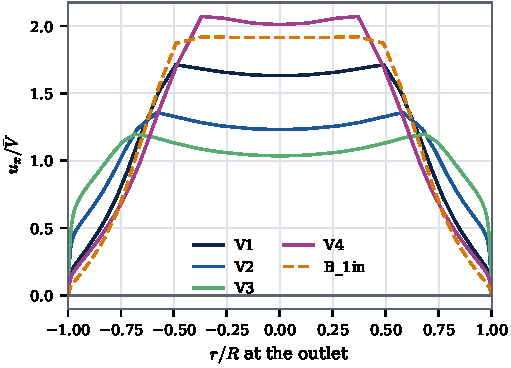
\includegraphics[width=\linewidth]{figures/outlet_profiles_30.pdf}\end{minipage}\hfill
\begin{minipage}{0.49\linewidth}\centering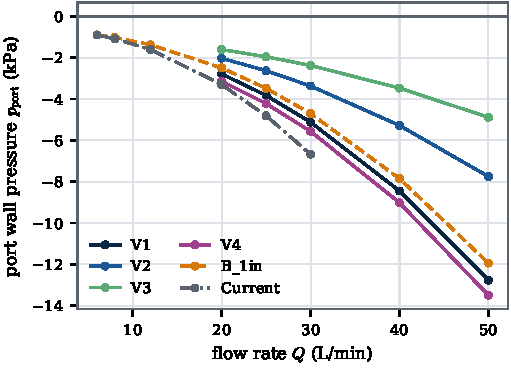
\includegraphics[width=\linewidth]{figures/port_vs_q.pdf}\end{minipage}
\caption{Left: axial velocity across the outlet at 30~L/min, normalised by the mean. Right: port wall pressure vs flow.}\label{fig:prof}
\end{figure}

\subsec{V1 against B\_1in: the effect of the diffuser angle alone}
V1 and B\_1in share the 14~mm throat and 26~mm exit; V1 has a 4$^\circ$ diffuser and B a 5$^\circ$ one (V1 also has no straight inlet). V1 needs 2.6~cm less level at 25~L/min and 3.3~cm less at 30~L/min (Table~\ref{tab:v1b}). The internal loss is the same within 0.1~cm. The gain comes from the outlet jet (lower $\alpha_o$ because the wall layer stays attached) and from V1's extra 0.85~cm of drop.

\begin{table}[htbp]\centering\small
\caption{V1 vs B\_1in at 25 and 30~L/min.}\label{tab:v1b}
\rowcolors{2}{white}{LB}
\begin{tabular}{|r|l|r|r|r|}
\hline
\thead\hd{$Q$} & \hd{Quantity} & \hd{B\_1in (5$^\circ$)} & \hd{V1 (4$^\circ$)} & \hd{V1 $-$ B}\\ \hline
25 & Level above inlet (cm) & 0.38 & -2.20 & -2.59\\ \hline
25 & Port wall pressure (kPa) & -3.476 & -3.822 & -0.347\\ \hline
25 & Diffuser recovery (--) & 0.815 & 0.870 & +0.055\\ \hline
25 & Reversed diffuser wall (fraction) & 0.52 & 0.00 & -0.52\\ \hline
25 & Outlet jet head (cm) & 8.08 & 6.29 & -1.79\\ \hline
25 & Outlet $\alpha$ & 2.58 & 2.00 & -0.57\\ \hline
25 & Internal loss (cm) & 3.95 & 4.01 & +0.06\\ \hline
25 & Drop inlet to outlet (cm) & 11.7 & 12.5 & +0.8\\ \hline
30 & Level above inlet (cm) & 5.12 & 1.83 & -3.29\\ \hline
30 & Port wall pressure (kPa) & -4.699 & -5.116 & -0.417\\ \hline
30 & Diffuser recovery (--) & 0.820 & 0.874 & +0.054\\ \hline
30 & Reversed diffuser wall (fraction) & 0.47 & 0.00 & -0.47\\ \hline
30 & Outlet jet head (cm) & 11.38 & 8.84 & -2.54\\ \hline
30 & Outlet $\alpha$ & 2.52 & 1.96 & -0.56\\ \hline
30 & Internal loss (cm) & 5.40 & 5.49 & +0.10\\ \hline
30 & Drop inlet to outlet (cm) & 11.7 & 12.5 & +0.8\\ \hline

\end{tabular}
\end{table}

\subsec{Chlorine port pressure}
Table~\ref{tab:port} splits the port pressure with Eq.~\eqref{eq:port}. At a given flow the Venturi part $p_V$ of V3 is about a third of V1's (at 20~L/min, $-0.63$ vs $-1.86$~kPa). V4's suction is the strongest because its throat matches V1 and its column below the port is 28~mm taller.

\begin{table}[htbp]\centering\small
\caption{Port wall pressure $p_\mathrm{port}$ and its Venturi part $p_V = p_\mathrm{port} + \rho g h_\mathrm{col}$ (kPa). Each flow column pair is $p_\mathrm{port}$ / $p_V$.}\label{tab:port}
\rowcolors{2}{white}{LB}
\begin{adjustbox}{max width=\linewidth}
\begin{tabular}{|l|r|r|r|r|r|r|r|r|r|r|r|r|}
\hline
\thead\hd{Design} & \hd{$h_\mathrm{col}$ (mm)} & \hd{$-\rho g h_\mathrm{col}$} & \multicolumn{2}{c|}{\hd{20 L/min}} & \multicolumn{2}{c|}{\hd{25 L/min}} & \multicolumn{2}{c|}{\hd{30 L/min}} & \multicolumn{2}{c|}{\hd{40 L/min}} & \multicolumn{2}{c|}{\hd{50 L/min}}\\ \hline
V1 & 94.4 & -0.92 & -2.78 & -1.86 & -3.82 & -2.90 & -5.12 & -4.19 & -8.44 & -7.52 & -12.76 & -11.84\\ \hline
V2 & 97.1 & -0.95 & -2.02 & -1.07 & -2.62 & -1.68 & -3.36 & -2.41 & -5.27 & -4.32 & -7.75 & -6.80\\ \hline
V3 & 99.9 & -0.98 & -1.60 & -0.63 & -1.95 & -0.97 & -2.37 & -1.40 & -3.47 & -2.49 & -4.88 & -3.91\\ \hline
V4 & 122.4 & -1.20 & -3.13 & -1.94 & -4.22 & -3.02 & -5.56 & -4.36 & -9.02 & -7.82 & -13.49 & -12.30\\ \hline
B\_1in & 77.2 & -0.75 & -2.49 & -1.73 & -3.48 & -2.72 & -4.70 & -3.94 & -7.85 & -7.09 & -11.93 & -11.18\\ \hline

\end{tabular}
\end{adjustbox}
\end{table}

% =====================================================================
\numsec{Discussion and what to watch}\label{sec:disc}

\subsec{Which part needs the least water level}
V3 needs the least level at every flow: $-9.2$~cm at 20~L/min, $-5.4$~cm at 30~L/min and $+6.2$~cm at 50~L/min, against $+5.1$ and $+31.1$~cm for B\_1in at 30 and 50~L/min. Its level reaches the inlet face only at about 40~L/min. Of the two parts that keep the 14~mm throat, V4 needs 3.6--7.5~cm less than V1 at every flow, and V1 needs the most of the set. These numbers exclude the reducer and elbow, which the bench tests show are close to their own limit; the allowance left for them is the 8.5~cm (Afridev) or 19~cm (India Mark~II) budget minus the values in the key-result table.

\subsec{Did the 4$^\circ$ diffuser fix B's separation?}
Yes, in this model. With the throat and exit unchanged, the 4$^\circ$ diffuser keeps the wall flow forward over its whole length at every flow, where B's 5$^\circ$ diffuser reverses over half of it. The benefit (2.6--3.3~cm at 25--30~L/min) is real but smaller than the separation pictures suggest, because the internal loss hardly changes; the gain is in the outlet jet. V1's wall shear falls to about 0.3~Pa at its exit, so any skew in the inflow (from the elbow) could tip the last part of the diffuser into separation. This needs the 3-D elbow runs (Stage 5).

\subsec{Chlorine suction and the dosing cutoff}
At 6--8~L/min the Venturi part of the port pressure is only $-0.1$ to $-0.4$~kPa in every design that was run there (Table~\ref{tab:portlow}); the remaining $-0.7$ to $-0.8$~kPa is the hanging column below the port. That column exists only while the bore below the port runs full of water. The bench result (dosing stops below about 6~L/min with the current part, and starts at 8~L/min with the printed B) is therefore most likely governed by whether the outlet runs full, which a single-phase, pipe-full model cannot predict. Stage 4 (volume-of-fluid) is the tool for that question.

\begin{table}[htbp]\centering\small
\caption{Port pressure at 6 and 8~L/min (kPa): total and Venturi part.}\label{tab:portlow}
\rowcolors{2}{white}{LB}
\begin{tabular}{|l|r|r|r|r|r|r|}
\hline
\thead\hd{Design} & \hd{$h_\mathrm{col}$ (mm)} & \hd{$-\rho g h_\mathrm{col}$} & \hd{$p_\mathrm{port}$, 6} & \hd{$p_V$, 6} & \hd{$p_\mathrm{port}$, 8} & \hd{$p_V$, 8}\\ \hline
Current & 69.0 & -0.67 & -0.90 & -0.22 & -1.08 & -0.41\\ \hline
A\_3-4in & 84.9 & -0.83 & -0.95 & -0.12 & -1.06 & -0.23\\ \hline
A\_1in & 77.2 & -0.75 & -0.88 & -0.12 & -0.98 & -0.23\\ \hline
B\_3-4in & 84.9 & -0.83 & -0.98 & -0.15 & -1.10 & -0.27\\ \hline
B\_1in & 77.2 & -0.75 & -0.89 & -0.14 & -1.01 & -0.26\\ \hline

\end{tabular}
\end{table}

What the CFD can say: at any flow where the pipe runs full, V2 and V3 produce less Venturi suction than V1 and V4, by a factor of about 1.7 (V2) and 3 (V3) at 20~L/min. If dosing near the 8~L/min cap depends on Venturi suction, V3 and V2 are the risky choices. Only a bench test of the printed parts can settle where each one starts to dose. An earlier informal estimate (scaling the 20~L/min suction with $Q^2$ to get dosing starts near 7, 8, 9 and 10~L/min) ignored the column term in Eq.~\eqref{eq:port} and should not be used.

\subsec{What to watch}
\begin{itemize}
\item \textbf{Negative inlet static pressure.} Every V-set part has $\bar{p}_1 < 0$ at 20--30~L/min (V2 and V3 also at 40~L/min); so do A and B at 20--25~L/min. The current part does not at 20~L/min and above. In service, a poorly sealed elbow-to-Venturi joint would draw air at these flows. Seal it.
\item \textbf{Exit non-uniformity.} $\alpha_o = 2.0$ (V1) and 2.5 (V4) means half of their jet energy is profile shape, not mean velocity. The cross-vanes (not modelled) may change this; a 3-D run with the vanes would show by how much.
\item \textbf{V1's marginal diffuser.} Near-zero wall shear at the exit makes it sensitive to inflow skew.
\item \textbf{Low-flow accuracy.} At 6--8~L/min the throat Reynolds number is about $10^4$; RANS results there carry more uncertainty than at the design flows.
\end{itemize}

% =====================================================================
\numsec{Assumptions and limitations}\label{sec:limits}
\begin{itemize}
\item Steady, single-phase, pipe-full flow. No free surface, no air, no unsteady pulsation from the piston. The outlet is assumed to run full at every flow.
\item 2-D axisymmetric: uniform, swirl-free inflow. The elbow's secondary flow and the skew it puts into the throat are absent. The chlorine port hole, the threads and the outlet cross-vane are not modelled.
\item The elbow, reducer and coupler losses are excluded; the reported level must be increased by $h_{L,\mathrm{up}}$.
\item $k$--$\omega$ SST with standard constants; separation onset in adverse pressure gradients is the most model-sensitive output. The reversed-wall lengths should be read as trends, not exact values.
\item Smooth walls. Printed parts have layer roughness; this raises loss and can move separation.
\item Mesh uncertainty on the level is about 2\% (one design, one flow).
\end{itemize}

% =====================================================================
\numsec{Recommendations and next steps}\label{sec:next}
\begin{enumerate}
\item \textbf{Bench-test the printed V1--V4} for inlet water level vs flow and for the flow at which dosing starts. Use V3 or V4 for the lowest level, but only if dosing still starts at or below 8~L/min.
\item \textbf{Upstream fittings.} The supplied eccentric reducer STEP (\texttt{3.5 inch eccentric reducer with npt 1 inch}) has a small-end thread of 26.67~mm OD with a 20.93~mm bore: standard 3/4" pipe, not 1". At 25--30~L/min a 20.9~mm passage is likely to cost more head than the bend. Confirm the printed part.
\item \textbf{Stage 5, 3-D:} reducer + bend + Venturi, half-domain with a symmetry plane, to get the bend loss, the throat skew, the port-side vs opposite-side throat pressure, and whether V1's diffuser stays attached behind a bend. Requires the bend geometry.
\item \textbf{Stage 4, volume-of-fluid} at 4--10~L/min to find where the outlet stops running full; this is the most likely control on the dosing cutoff.
\item \textbf{Stage 6:} feed the CFD level-vs-flow curves into a stroke-by-stroke tank model once stroke volume and pumping rate are measured.
\end{enumerate}

% =====================================================================
\begin{landscape}
\thispagestyle{empty}
\docbannerS{Appendix A: Every Run}{54 single-phase runs \textbullet{} medium mesh unless noted \textbullet{} shaded: inlet static pressure below atmospheric}
{\scriptsize\setlength{\tabcolsep}{2.6pt}\renewcommand{\arraystretch}{1.12}
\rowcolors{2}{white}{LB}
\begin{longtable}{|l|r|r|r|r|r|r|r|r|r|r|r|r|r|r|r|r|}
\hline
\thead\hd{Case} & \hd{$Q$} & \hd{Cells} & \hd{$h$ (cm)} & \hd{$\bar p_{t,1}$ (Pa)} & \hd{$\bar p_1$ (Pa)} & \hd{$p_\mathrm{port}$ (kPa)} & \hd{min $p_w$ (kPa)} & \hd{$C_p$} & \hd{$\eta_d$} & \hd{$\epsilon_\mathrm{rev}$ (\%)} & \hd{$h_{KE}$ (cm)} & \hd{$\alpha_o$} & \hd{$h_L$ (cm)} & \hd{$y^+_\mathrm{max}$} & \hd{$p$ res.} & \hd{$\epsilon_m$}\\ \hline
\endfirsthead
\hline
\thead\hd{Case} & \hd{$Q$} & \hd{Cells} & \hd{$h$ (cm)} & \hd{$\bar p_{t,1}$ (Pa)} & \hd{$\bar p_1$ (Pa)} & \hd{$p_\mathrm{port}$ (kPa)} & \hd{min $p_w$ (kPa)} & \hd{$C_p$} & \hd{$\eta_d$} & \hd{$\epsilon_\mathrm{rev}$ (\%)} & \hd{$h_{KE}$ (cm)} & \hd{$\alpha_o$} & \hd{$h_L$ (cm)} & \hd{$y^+_\mathrm{max}$} & \hd{$p$ res.} & \hd{$\epsilon_m$}\\ \hline
\endhead
Current & 6 & 53040 & -9.70 & -949 & \cellcolor{StProg}-986 & -0.898 & -1.036 & 0.410 & 0.694 & 85 & 1.35 & 1.42 & 0.60 & 0.31 & 4.7e-08 & -7e-10\\ \hline
Current & 8 & 53040 & -8.39 & -821 & \cellcolor{StProg}-887 & -1.080 & -1.247 & 0.424 & 0.718 & 72 & 2.31 & 1.37 & 0.95 & 0.37 & 9.4e-08 & -1e-10\\ \hline
Current & 12 & 53040 & -4.78 & -468 & \cellcolor{StProg}-618 & -1.599 & -1.877 & 0.442 & 0.748 & 25 & 5.01 & 1.32 & 1.86 & 0.50 & 1.9e-07 & -1e-09\\ \hline
Current & 20 & 53040 & 6.21 & 608 & 190 & -3.295 & -4.016 & 0.460 & 0.779 & 0 & 13.38 & 1.27 & 4.48 & 0.72 & 2.8e-07 & -3e-09\\ \hline
Current (fine) & 25 & 114480 & 15.61 & 1527 & 875 & -4.800 & -5.971 & 0.467 & 0.791 & 0 & 20.62 & 1.25 & 6.64 & 0.63 & 4.9e-08 & -2e-11\\ \hline
Current (coarse) & 25 & 25380 & 15.42 & 1508 & 856 & -4.814 & -5.979 & 0.469 & 0.794 & 0 & 20.55 & 1.24 & 6.52 & 1.12 & 1.2e-06 & -3e-10\\ \hline
Current & 25 & 53040 & 15.53 & 1519 & 867 & -4.806 & -5.981 & 0.468 & 0.792 & 0 & 20.59 & 1.25 & 6.59 & 0.84 & 4.9e-07 & -2e-09\\ \hline
Current & 30 & 53040 & 26.68 & 2610 & 1671 & -6.666 & -8.445 & 0.474 & 0.802 & 0 & 29.30 & 1.23 & 9.03 & 0.96 & 6.8e-07 & -2e-09\\ \hline
A\_3-4in & 6 & 48160 & -10.44 & -1021 & \cellcolor{StProg}-1063 & -0.954 & -1.065 & 0.499 & 0.710 & 89 & 0.82 & 1.29 & 0.39 & 0.27 & 3.6e-08 & -1e-10\\ \hline
A\_3-4in & 8 & 48160 & -9.66 & -945 & \cellcolor{StProg}-1019 & -1.058 & -1.142 & 0.536 & 0.763 & 90 & 1.41 & 1.25 & 0.58 & 0.33 & 5.6e-08 & 5e-11\\ \hline
A\_3-4in & 12 & 48160 & -7.51 & -734 & \cellcolor{StProg}-900 & -1.356 & -1.490 & 0.559 & 0.796 & 34 & 3.05 & 1.20 & 1.09 & 0.44 & 9.1e-08 & -2e-10\\ \hline
A\_3-4in & 20 & 48160 & -0.90 & -88 & \cellcolor{StProg}-549 & -2.299 & -2.625 & 0.578 & 0.822 & 4 & 8.21 & 1.17 & 2.54 & 0.63 & 1.6e-07 & -4e-11\\ \hline
A\_3-4in & 25 & 48160 & 4.72 & 462 & \cellcolor{StProg}-260 & -3.138 & -3.637 & 0.585 & 0.833 & 0 & 12.67 & 1.15 & 3.70 & 0.74 & 1.8e-07 & -2e-11\\ \hline
A\_3-4in & 30 & 48160 & 11.47 & 1121 & 83 & -4.172 & -4.885 & 0.591 & 0.842 & 0 & 18.08 & 1.14 & 5.03 & 0.85 & 2.1e-07 & 1e-11\\ \hline
A\_1in & 6 & 48160 & -10.41 & -1019 & \cellcolor{StProg}-1035 & -0.875 & -1.034 & 0.467 & 0.666 & 90 & 0.85 & 1.33 & 0.39 & 0.24 & 4.5e-08 & 3e-09\\ \hline
A\_1in & 8 & 48160 & -9.64 & -943 & \cellcolor{StProg}-971 & -0.980 & -1.064 & 0.523 & 0.744 & 91 & 1.44 & 1.28 & 0.57 & 0.30 & 6.7e-08 & -1e-09\\ \hline
A\_1in & 12 & 48160 & -7.55 & -738 & \cellcolor{StProg}-803 & -1.284 & -1.417 & 0.561 & 0.799 & 36 & 3.09 & 1.22 & 1.01 & 0.40 & 1.0e-07 & 2e-10\\ \hline
A\_1in & 20 & 48160 & -1.01 & -99 & \cellcolor{StProg}-278 & -2.234 & -2.555 & 0.578 & 0.823 & 5 & 8.29 & 1.18 & 2.35 & 0.57 & 4.1e-07 & -2e-09\\ \hline
A\_1in & 25 & 48160 & 4.57 & 447 & 167 & -3.067 & -3.569 & 0.585 & 0.833 & 0 & 12.79 & 1.16 & 3.43 & 0.67 & 3.8e-07 & -3e-10\\ \hline
A\_1in & 30 & 48160 & 11.27 & 1102 & 698 & -4.098 & -4.819 & 0.591 & 0.841 & 0 & 18.25 & 1.15 & 4.67 & 0.76 & 4.2e-07 & -5e-10\\ \hline
B\_3-4in & 6 & 48160 & -10.66 & -1043 & \cellcolor{StProg}-1084 & -0.975 & -1.087 & 0.682 & 0.746 & 95 & 0.54 & 2.97 & 0.45 & 0.27 & 1.9e-08 & 0e+00\\ \hline
B\_3-4in & 8 & 48160 & -10.09 & -987 & \cellcolor{StProg}-1061 & -1.100 & -1.184 & 0.709 & 0.775 & 96 & 0.89 & 2.76 & 0.67 & 0.33 & 2.9e-08 & -5e-11\\ \hline
B\_3-4in & 12 & 48160 & -8.53 & -834 & \cellcolor{StProg}-1000 & -1.456 & -1.590 & 0.725 & 0.793 & 73 & 1.86 & 2.57 & 1.27 & 0.44 & 3.0e-08 & -7e-11\\ \hline
B\_3-4in & 20 & 48160 & -3.87 & -378 & \cellcolor{StProg}-840 & -2.590 & -2.915 & 0.741 & 0.809 & 58 & 4.81 & 2.39 & 2.97 & 0.63 & 5.7e-08 & -9e-11\\ \hline
B\_3-4in & 25 & 48160 & -0.01 & -1 & \cellcolor{StProg}-723 & -3.601 & -4.100 & 0.747 & 0.817 & 51 & 7.30 & 2.33 & 4.34 & 0.74 & 6.1e-08 & 5e-11\\ \hline
B\_3-4in & 30 & 48160 & 4.54 & 444 & \cellcolor{StProg}-595 & -4.849 & -5.562 & 0.753 & 0.822 & 46 & 10.28 & 2.27 & 5.92 & 0.85 & 7.0e-08 & 0e+00\\ \hline
B\_1in & 6 & 48160 & -10.58 & -1035 & \cellcolor{StProg}-1051 & -0.892 & -1.050 & 0.659 & 0.720 & 96 & 0.62 & 3.45 & 0.45 & 0.24 & 5.2e-08 & 3e-09\\ \hline
B\_1in & 8 & 48160 & -9.99 & -977 & \cellcolor{StProg}-1006 & -1.014 & -1.098 & 0.699 & 0.763 & 96 & 1.01 & 3.14 & 0.65 & 0.30 & 4.0e-08 & -8e-10\\ \hline
B\_1in & 12 & 48160 & -8.43 & -825 & \cellcolor{StProg}-889 & -1.371 & -1.503 & 0.727 & 0.794 & 73 & 2.06 & 2.85 & 1.16 & 0.40 & 5.4e-08 & -1e-09\\ \hline
B\_1in & 20 & 48160 & -3.62 & -354 & \cellcolor{StProg}-534 & -2.489 & -2.811 & 0.739 & 0.808 & 59 & 5.32 & 2.65 & 2.70 & 0.57 & 1.3e-07 & 1e-09\\ \hline
B\_1in & 25 & 48160 & 0.38 & 38 & \cellcolor{StProg}-243 & -3.476 & -3.979 & 0.746 & 0.815 & 52 & 8.08 & 2.58 & 3.95 & 0.67 & 1.3e-07 & -2e-11\\ \hline
B\_1in & 30 & 48160 & 5.12 & 501 & 98 & -4.699 & -5.420 & 0.751 & 0.820 & 47 & 11.38 & 2.52 & 5.40 & 0.76 & 1.5e-07 & 4e-10\\ \hline
B\_1in & 40 & 48160 & 16.73 & 1636 & 919 & -7.847 & -9.131 & 0.759 & 0.829 & 38 & 19.53 & 2.43 & 8.85 & 0.93 & 2.6e-07 & -2e-10\\ \hline
B\_1in & 50 & 48160 & 31.08 & 3040 & 1919 & -11.933 & -13.947 & 0.765 & 0.836 & 30 & 29.72 & 2.37 & 13.00 & 1.09 & 3.3e-07 & -9e-11\\ \hline
V1 & 20 & 51520 & -5.62 & -550 & \cellcolor{StProg}-644 & -2.780 & -3.118 & 0.791 & 0.865 & 0 & 4.15 & 2.07 & 2.73 & 0.56 & 3.1e-07 & -1e-08\\ \hline
V1 & 25 & 51520 & -2.20 & -216 & \cellcolor{StProg}-364 & -3.822 & -4.359 & 0.796 & 0.870 & 0 & 6.29 & 2.00 & 4.01 & 0.65 & 3.6e-07 & 1e-08\\ \hline
V1 & 30 & 51520 & 1.83 & 179 & \cellcolor{StProg}-34 & -5.116 & -5.889 & 0.800 & 0.874 & 0 & 8.84 & 1.96 & 5.49 & 0.74 & 3.4e-07 & -9e-09\\ \hline
V1 & 40 & 51520 & 11.70 & 1144 & 765 & -8.444 & -9.822 & 0.807 & 0.882 & 0 & 15.14 & 1.88 & 9.06 & 0.91 & 3.8e-07 & -2e-09\\ \hline
V1 & 50 & 51520 & 23.87 & 2335 & 1743 & -12.759 & -14.916 & 0.812 & 0.887 & 0 & 23.00 & 1.83 & 13.37 & 1.07 & 4.3e-07 & 9e-09\\ \hline
V2 & 20 & 51440 & -8.14 & -796 & \cellcolor{StProg}-891 & -2.025 & -2.270 & 0.754 & 0.881 & 0 & 2.77 & 1.38 & 1.58 & 0.49 & 1.2e-07 & -8e-10\\ \hline
V2 & 25 & 51440 & -5.96 & -583 & \cellcolor{StProg}-731 & -2.625 & -3.003 & 0.759 & 0.887 & 0 & 4.22 & 1.34 & 2.32 & 0.57 & 1.5e-07 & 3e-10\\ \hline
V2 & 30 & 51440 & -3.37 & -329 & \cellcolor{StProg}-543 & -3.364 & -3.908 & 0.763 & 0.892 & 0 & 5.95 & 1.32 & 3.18 & 0.65 & 1.4e-07 & 9e-10\\ \hline
V2 & 40 & 51440 & 3.01 & 294 & \cellcolor{StProg}-85 & -5.273 & -6.232 & 0.770 & 0.900 & 0 & 10.27 & 1.28 & 5.23 & 0.80 & 2.0e-07 & -4e-09\\ \hline
V2 & 50 & 51440 & 10.94 & 1070 & 478 & -7.745 & -9.241 & 0.776 & 0.907 & 0 & 15.72 & 1.25 & 7.72 & 0.94 & 1.9e-07 & -9e-11\\ \hline
V3 & 20 & 51440 & -9.18 & -898 & \cellcolor{StProg}-993 & -1.603 & -1.796 & 0.692 & 0.900 & 0 & 2.30 & 1.15 & 1.02 & 0.43 & 1.1e-07 & 2e-10\\ \hline
V3 & 25 & 51440 & -7.47 & -730 & \cellcolor{StProg}-878 & -1.949 & -2.238 & 0.697 & 0.907 & 0 & 3.54 & 1.13 & 1.49 & 0.51 & 1.6e-07 & 2e-10\\ \hline
V3 & 30 & 51440 & -5.41 & -529 & \cellcolor{StProg}-743 & -2.372 & -2.782 & 0.701 & 0.912 & 0 & 5.04 & 1.12 & 2.04 & 0.58 & 2.0e-07 & 5e-10\\ \hline
V3 & 40 & 51440 & -0.29 & -29 & \cellcolor{StProg}-408 & -3.466 & -4.179 & 0.707 & 0.919 & 0 & 8.83 & 1.10 & 3.37 & 0.71 & 2.6e-07 & 2e-09\\ \hline
V3 & 50 & 51440 & 6.15 & 602 & 10 & -4.882 & -5.988 & 0.711 & 0.925 & 0 & 13.66 & 1.09 & 4.99 & 0.84 & 3.3e-07 & 5e-10\\ \hline
V4 & 20 & 62560 & -9.22 & -902 & \cellcolor{StProg}-996 & -3.132 & -3.470 & 0.827 & 0.868 & 3 & 2.99 & 2.64 & 3.09 & 0.56 & 2.5e-07 & -2e-08\\ \hline
V4 & 25 & 62560 & -6.23 & -609 & \cellcolor{StProg}-757 & -4.216 & -4.753 & 0.831 & 0.872 & 0 & 4.53 & 2.56 & 4.54 & 0.65 & 3.4e-07 & -2e-08\\ \hline
V4 & 30 & 62560 & -2.71 & -265 & \cellcolor{StProg}-478 & -5.560 & -6.333 & 0.834 & 0.876 & 0 & 6.37 & 2.50 & 6.22 & 0.74 & 4.0e-07 & -2e-08\\ \hline
V4 & 40 & 62560 & 5.85 & 572 & 193 & -9.016 & -10.394 & 0.840 & 0.883 & 0 & 10.90 & 2.40 & 10.25 & 0.91 & 4.4e-07 & -5e-09\\ \hline
V4 & 50 & 62560 & 16.37 & 1601 & 1009 & -13.492 & -15.650 & 0.845 & 0.888 & 0 & 16.55 & 2.34 & 15.12 & 1.07 & 4.1e-07 & -2e-09\\ \hline

\end{longtable}}
\landfooter
\end{landscape}

% =====================================================================
\sectionhead{Appendix B: files, scripts and viewer}
\begin{center}\small\rowcolors{2}{white}{LB}
\begin{tabular}{|p{0.36\linewidth}|p{0.56\linewidth}|}
\hline
\thead\hd{File} & \hd{Purpose}\\ \hline
\texttt{cfd/make\_wedge\_mesh.py} & structured wedge mesh from \texttt{geometry/bore\_stations.csv} \\ \hline
\texttt{cfd/setup\_case.py} & writes one OpenFOAM case (fields, physics, schemes) \\ \hline
\texttt{cfd/run\_case.sh} & stages a case in WSL, runs \texttt{checkMesh} and \texttt{foamRun}, copies results back \\ \hline
\texttt{cfd/postprocess.py} & every quantity in Section~\ref{sec:derive} \\ \hline
\texttt{cfd/make\_results\_csv.py} & results CSVs in \texttt{cfd/results/} \\ \hline
\texttt{cfd/viz\_axisym.py}, \texttt{cfd/build\_gui\_data.py} & field data and pictures for the viewer \\ \hline
\texttt{report/make\_report\_assets.py} & every table and figure in this report \\ \hline
\texttt{cfd/results/venturi\_set\_stage3b.csv} & Stage 3b results \\ \hline
\end{tabular}\end{center}
Interactive viewer (all 54 runs, 3-D views, probes, particle tracing, line and sweep plots): \Rl{https://kamronsoltani.github.io/Venturi-Redesign/}.

\vspace{6pt}
\sectionhead{Revision history}
\rowcolors{2}{white}{LB}
{\renewcommand{\arraystretch}{1.7}
\begin{longtable}{|p{0.09\wFour}|p{0.17\wFour}|p{0.22\wFour}|p{0.52\wFour}|}
\hline
\rowcolor{Navy}\hd{Rev}&\hd{Date}&\hd{Author}&\hd{Changes}\\
\hline
\revrow{1}{Nov 16, 2026}{Kamron Soltani}{Initial release: Stages 1, 3 and 3b.}
\revrow{}{}{}{}
\revrow{}{}{}{}
\end{longtable}}

\end{document}
